\documentclass[10pt]{article}
\usepackage[utf8]{inputenc}
\usepackage[english,russian]{babel}
\usepackage[T2A]{fontenc}
\usepackage{graphics}
\usepackage{graphicx}
\usepackage{amsmath,amssymb,amsthm,amsfonts,amscd}
\usepackage{float}
\usepackage{subfig}
\usepackage{algorithm}
\usepackage[noend]{algpseudocode}
\usepackage{hyperref}
\captionsetup[algorithm]{labelformat=empty}

\newtheorem{thm}{\indent Теорема}
\newtheorem{lem}{\indent Лемма}
\newtheorem{prop}{\indent Утверждение}
\bibliographystyle{unsrt}
\graphicspath{{../optimization/results/}}

\begin{document}
    \section{Введение}\label{sec:intro}
    Стационарная нормализированная диффузионная модель, описывающая радиационный и кондуктивный
    обмен в ограниченной области $\Omega \subset \mathbb{R}^3$ имеет следующий вид~\cite{modest-rht}
    \begin{equation}
        \label{initial}
        \begin{aligned}
            - a \Delta \theta + b \kappa_a(\theta ^ 3 | \theta | - \varphi) = 0,  \\
            - \alpha \Delta \varphi + \kappa_a (\varphi - \theta ^3 | \theta |) = 0.
        \end{aligned}
    \end{equation}
    Здесь $\theta$ – нормализованная температура,
    $\varphi$ – нормализованная интенсивность излучения, усредненная по всем направлениям.
    Положительные физические параметры $a, b, \kappa_a $ и $\alpha$,
    описывающие свойства среды, определяются стандартным образом~\cite{covt-cheb-unique}.

    Далее будем считать, что функция $\theta$ удовлетворяет следующему условию на границе
    $\Gamma = \partial \Omega$:
    \begin{equation}
        \label{theta_boundary_dirichlet}
        \theta|_\Gamma = \theta_b.
    \end{equation}
    Для задания сдандартного краевого условия для интенсивности излучения $\phi$ обычно
    используют граничное условие вида
    \begin{equation}
        \label{phi_boundary_default}
        - \alpha \partial_n \varphi + \gamma (\varphi - \theta ^4) = 0.
    \end{equation}
    здесь и далее $\partial_n$ обозначает производную в отношении внешней нормали.
    В случае если функция $\gamma$ не известна, естественно вместо краевого условия для
    интенсивности излучения задать значение теплового потока на границе
    \begin{equation}
        \label{theta_boundary_neumann}
        \partial_n \theta = q_b.
    \end{equation}
    В данной работе представлен численный алгоритм для решения краевой
    задачи~\eqref{initial},~\eqref{theta_boundary_dirichlet},~\eqref{theta_boundary_neumann},
    на которую мы будем ссылаться как на задачу $P$.
    Зная решение указанной задачи, можно вычислить
    неизвестную функцию $\gamma$, используя уравнение~\eqref{phi_boundary_default}.
    Теоретический анализ задачи $P$ можно найти в~\cite{cheb_same}.
    Исследование математических моделей радиационного теплопереноса [1], учитывающих одновременно
    вклад эффектов теплопроводности и излучения даёт теоре-тическую основу для инженерных решений
    в различных областях, таких как произ-водство стекла [2],
    лазерная интерстициальная термотерапия [3], и др.
    Главной особенностью данных процессов является существенное влияние излучения на теплообмен
    при высоких температурах.
    Значительное число работ посвящено исследованиюзадач управления для
    нестационарных моделей сложного теплообмена [4–6], в ко-торых для описания температурного поля
    используется нестационарное уравнениетеплопроводности, а для моделирования излучения --
    стационарное диффузионноеприближение уравнения переноса излучения.
    В работах [7, 8] задача оптимального управления сводится к
    bang-bang принципу [9], или аналогичному.
    Близкие крассмотренной в данной статье, задача управления коэффициентом отражения
    для полностью стационарной модели исследовалась в [10],
    для нестационарной модели – в [11].
    Отметим также работы [12, 13], в которых рассмотрены свойства квазирешений
    обратных задач для уравнений тепломассапереноса.

    \section{Формализация задачи нахождения квазирешения}\label{sec:formalization}

    Будем предполагать что исходные данные удовлетворяют следующему условию:

    %    TODO: ПЕРЕПИСАТЬ

    (i) $\beta\in L^\infty(\Gamma);\; \gamma \in L^\infty(\Gamma_0\cup\Gamma_2);\;
    u_1, u_2 \in L^\infty(\Gamma_1);
    \; 0 < \beta_0 \le \beta;\;  0 < \gamma_0 \le \gamma; \;
    \beta_0,\gamma_0=Const,\;\;\\ 0 \le u_1 \le u_2;$

    Пусть $H = L^2(\Omega), V = W^1_2(\Omega), Y = V \times V $.
    Пространство $H$ отождествляем с сопряжённым пространством $H'$ так,
    что $V \subset H = H' \subset V'$.
    Определим $(f,v)$ как значение функционала $f \in V'$ на элементе $v \in V$,
    совпадающее со скалярным произведением в $H$, если $f\in H, \|f\|^2 = (f,f)$.
    Пространство $U = L^2(\Gamma_1)$ является пространством управлений;
    $U_{ad} = \{u \in U, u_1 \le u \le u_2 \}$ --- множество допустимых управлений.

    Пусть $v$ произвольный элемент множества $H^1(\Omega)$.
    Определим операторы:

    \begin{gather*}
        A_{1,2}\colon V \to V', \;\; F \colon V \times U \to V', \; f \in V', \; g \in V'.\\
        (A_1\theta,v) = a( \nabla \theta, \nabla v ) + \int_\Gamma \beta \theta v d\Gamma, \;
        (A_2 \varphi, v) = \alpha (\nabla \varphi,\nabla v)
        + \int_{\Gamma_0 \cup \Gamma_2} \gamma \varphi v d\Gamma,\\
        (f,v) = \int_\Gamma \beta \theta_b v d\Gamma, \; \;
        (g,v) = \int_{\Gamma_0 \cup \Gamma_2} \gamma \theta_b^4 v d\Gamma,\\
        (F(\varphi, u), v) = \int_{\Gamma_1} u (\varphi - \theta^4_b)v d\Gamma.\\
    \end{gather*}

    Пару $\{\theta, \varphi \} \in Y$ будем называть слабым решением
    задачи~\eqref{initial},~\eqref{initial_boundary}, если
    \begin{equation}
        \label{weak_operational}
        A_1 \theta + b \kappa_a (| \theta | \theta^3 - \varphi ) = f,
        A_2 \varphi + \kappa_a (\varphi - |\theta|\theta^3) + F(\varphi, u) = g.
    \end{equation}

    Задача нахождения квазирешения состоит в минимизации функционала $J(\theta, u)$,
    определённом на компоненте $\theta$ решения системы~\eqref{weak_operational}.
    Таким образом
    \begin{equation}
        \label{minimization_operational}
        J(\theta, u) \to \text{inf}, \; \{\theta, \varphi\}
        \text{ решение~\eqref{weak_operational}, соответствующее функции }
        u \in U_{ad}.
    \end{equation}


    Пара $\{\hat{\theta}, \hat{\varphi} \}$ соответствующая минимуму $J$,
    отвечающая функции $\hat{u}$ называется оптимальным состоянием.
    В таком случае $\hat{u}$ называется квазирешением
    обратной задачи~\eqref{initial}--\eqref{theta_gamma}.

    \section{Анализ решения экстремальной задачи}\label{sec:analysis}

    Для доказательства разрешимости задачи~\eqref{minimization_operational} нам необходимо также
    установить некоторые свойства решения задачи~\eqref{initial},~\eqref{initial_boundary}.

    \begin{lem}[\cite{lemma_proof}]
        \label{SolvabilityLemma}
        Пусть выполняется условие (i).
        Тогда для каждого $ u \in U_{ad} $ существует единственное
        слабое решение $\{\theta, \varphi \}$ для задачи~\eqref{initial},~\eqref{initial_boundary}
        и справедливы оценки:
        \begin{equation}
            \label{lemma_1}
            M_1 \le \theta \le M_2, \; M_1^4 \le \varphi \le M_2^4,
        \end{equation}
        \begin{equation}
            \label{lemma_2}
            \| \nabla \varphi \|^2 \le C.
        \end{equation}
        Здесь $M_1 = \text{ess inf } \theta_b, M_2 = \text{ess sup } \theta_b$,
        и константа $C > 0$ зависит только от \\
        $a, b, \alpha, \kappa_a, \beta, \gamma, \|u\|_{L^\infty(\Gamma)}$ и области $\Omega$.
    \end{lem}


    Для вывода системы оптимальности, покажем дифференцируемость функционала $J$.
    \begin{lem}
        \label{freshet_diff}
        Функционал $J : V \rightarrow \mathbb{R}$ дифференцируем по Фреше.
    \end{lem}
    \begin{proof}
        Покажем, что для произвольной функции $\theta \in V$ выполняется следующее равенство:
        \begin{equation}
            \label{lemma_proof_1}
            J(\theta + h) = J(\theta) + J'(\theta)\langle h \rangle + r(\theta, h) \;
            \forall h \in V, \; \text{ где } \;
            J'(\theta)\langle h \rangle = \int_{\Gamma_2} (\theta - \theta_0)h d\Gamma,
        \end{equation}
        где для остаточного члена $r(\theta,h)$ справедливо соотношение:
        \begin{equation}
            \label{lemma_proof_2}
            \frac{|r(\theta,h)|}{\|h\|_V} \rightarrow 0 \quad \text{при}
            \quad \|h\|_V \rightarrow 0.
        \end{equation}
        Перепишем \eqref{lemma_proof_1} в виде
        \[
            \frac{1}{2} \|\theta + h - \theta_0\|^2_{L^2(\Gamma_2)} =
            \frac{1}{2} \| \theta - \theta_0 \|^2_{L^2(\Gamma_2)} +
            (\theta - \theta_0, h)_{L^2(\Gamma_2)} +
            \frac{1}{2}\| h \|^2_{L^2(\Gamma_2)}.
        \]
        Согласно теореме о следах $ \|h\|_{L^2(\Gamma_2)} \le C \|h\|_V $,
        где $C$ не зависит от $h$.
        Поэтому
        \[
            \frac{r(\theta,h)}{\| h \|_V} \leq
            \frac{1}{2} C^2 \| h \|_V \rightarrow 0 \quad \text{при } \| h \|_V \rightarrow 0.
        \]
    \end{proof}

    Вывод условий оптимальности основан на принципе множителей
    Лагранжа для гладко-выпуклых задач минимизации.
    \begin{thm}
        \label{adjoint_theorem}
        Пусть $\hat{y}=\{\hat{\theta},\hat{\varphi} \} \in Y, \hat{u} \in U_{ad}$ --- решение
        экстремальной задачи \eqref{minimization_operational}.
        Тогда существует пара $p = (p_1, p_2)$, $p \in Y$
        такая, что тройка $(\hat{y}, \hat{u}, p)$, удовлетворяет следующим условиям:
        \begin{equation}
            \label{theorem_2_eq1}
            A_1 p_1 + 4 |\hat{\theta}|^3 \kappa_a(b p_1 - p_2) = f_c, \;\;
            (f_c,v) = - \int_{\Gamma_2} (\hat{\theta} - \theta_0) v d\Gamma,
        \end{equation}
        \begin{equation}
            \label{theorem_2_eq2}
            A_2 p_2 + \kappa_a (p_2-b p_1) = g_c(( p_2, \hat{u}),v), \;\;
            g_c(( p_2, \hat{u}),v) = -\int_{\Gamma_1} \hat{u} p_2 v\Gamma,
        \end{equation}
        \begin{equation}
            \label{theorem_2_eq3}
            \int_{\Gamma_1} p_2 (\hat{\varphi} - \theta_b^4)(u-w) \leq 0
            \quad \forall w \in U_{ad}.
        \end{equation}
    \end{thm}
    \begin{proof}
        Перепишем уравнения~\eqref{weak_operational} следующим образом:
        \begin{gather*}
            H(y,u) = 0,\;\; y = \{\theta,\varphi\} \in Y, \; \text{где}\\
            H:Y \times U \to Y',\\
            H(y,u) =\{A_1 \theta + b \kappa_a (| \theta | \theta^3 - \varphi ) - f,
            A_2 \varphi + \kappa_a (\varphi - |\theta|\theta^3) + F(\varphi, u) - g \}.\\
        \end{gather*}
        Заметим, что для всех $u \in U_{ad}$, отображение $y \to J(\theta) $ и $y \to H(y,u)$
        непрерывно дифференцируемо в окрестности $\mathcal{O}(\hat{y})$ точки $\hat{y}$.
        Непрерывная дифференцируемость членов в $H$ следует из непрерывной дифференцируемости
        функции $t \in \mathbb{R} \to | t | t^3$, а также из непрерывности вложения
        $V \subset L^6(\Omega)$.
        В дополнение, отображение $u \to H(y,u)$ непрерывно из $U \to Y'$ и афинно.
        В~\cite{cheb_origin} показано, что $\text{Im}H_y'(\hat{y}, \hat{u}) = Y$,
        что влечёт невырожденность условий оптимальности.

        Рассмотрим функцию Лагранжа
        $L(y,u,p) = J(\theta) + (H(y,u),p)$, где $y,p \in Y,\, u \in U_{ad}$.
        Согласно принципу Лагранжа \cite[Гл.2, Теорема 1.5]{theorem_proof_18}
        существует пара $p = \{p_1,p_2\} \in Y$ такая, что
        \begin{equation}
            \label{th2_proof_1}
            (L_\theta,\zeta) =\int_{\Gamma_2}(\hat\theta -\theta_0) \zeta d\Gamma +
            (A_1 \zeta + 4b\kappa_a |\hat\theta|^3 \zeta,p_1) -
            4\kappa_a(|\hat\theta|^3 \zeta,p_2) = 0 \; \forall \zeta \in V,
        \end{equation}
        \begin{equation}
            \label{th2_proof_2}
            (L_\varphi, \zeta) = (A_2 \zeta + \kappa_a \zeta, p_2) -
            b \kappa_a(\zeta,p_1) +\int_{\Gamma_1} \hat u \zeta p_2 = 0 \; \forall \zeta \in V,
        \end{equation}
        \begin{equation}
            \label{th2_proof_3}
            (L_u,\tau) = \int_{\Gamma_1} \tau (\varphi - \theta^4_b) p_2 d\Gamma  \leq 0, \;
            \tau := \hat u - w \; \forall w \in U_{ad}.
        \end{equation}
        Сопряжённые уравнения~\eqref{theorem_2_eq1},~\eqref{theorem_2_eq2} являются прямым
        следствием вариационных равенств~\eqref{th2_proof_1} и~\eqref{th2_proof_2}.
    \end{proof}

    \section{Численные эксперименты}\label{sec:experiments}

    Пусть функционал $J(\theta)$ удовлетворяет условиям, указанным в \autoref{sec:optimality}.
    Для удобства введём переобозначение
    $\hat{J}(u):=J(\theta(u)), \hat{J}:L^2(\Gamma_1) \to \mathbb{R}$.
    Здесь $\theta(u)$ -- температурное поле задачи~\eqref{initial}--\eqref{initial_boundary}
    отвечающее управлению $u \in L^2(\Gamma_1)$.
    Согласно формуле~\eqref{theorem_2_eq3} градиент функционала $\hat{J}(u)$~\cite{grenkin_13}
    имеет вид \[ hat{J}'(u)= (\varphi(u) -\theta_b^4)p_2 \],
    где $\varphi(u)$ есть интенсивность излучения,
    $p_2$ -- соответствующая переменная сопряжённой системы.

    Предлагаемый алгоритм решения выглядит следующим образом:
    %    \begin{algorithm}[H]
    %        \caption{Алгоритм градиентного спуска с проекцией}
    %        \begin{algorithmic}[1]
    %            \State Выбираем значение градиентного шага $\lambda$,
    %            \State Выбираем количество итераций $N$,
    %            \State Выбираем произвольное $u_0 \in U_{ad}$,
    %            \For{$k \gets 0,1,2,\ldots,N$}:
    %            \State Для полученного $u_k$ расчитываем состояние
    % $y_k = \{\theta_k, \va\eqref{weak_operational} (\ref{weak_operational}).
    %            \State Расчитываем значение функционала качества $J(\theta_k)$ из (\ref{quality}).
    %            \State Расчитываем сопряжённое состояние $p_k=\{p_{1k},p_{2k}\}$ из
    %            уравнений~\eqref{therorem_2_eq1}--\eqref{therorem_2_eq2},
    %            где $ \hat{\theta} := \theta_k, \hat{u}=u_k$.
    %            \State Пересчитываем управление
    %            $u_{k+1} = P_{ad}\left[ u_k - \lambda (\varphi_k - \theta_b^4)p_{2k} \right]$.
    %            \EndFor
    %        \end{algorithmic}
    %    \end{algorithm}
    Приведём далее примеры расчётов для двумерного случая.
    Положим $\Omega = \{(x,y), 0 \leq x,y \leq 1\}$, $l = 1$ см.
    Будем далее считать, что $a = 0.006[\text{см}^2/\text{c}]$, $b=0.025[\text{см}/\text{с}]$,
    $\beta = 0.00005[\text{см}/\text{с}]$, $\kappa=1[\text{см}^{-1}]$, $\kappa_s = 0$, $A = 0$,
    $\gamma = 0.3$.
    Указанные параметры соответствуют стеклу~\cite{grenkin_13}.
    Температуру на границе $\Omega$ положим равной $\theta_b = (x^2+y^2)/3$.

    При указанных параметрах для первого эксперимента выберем следующее тестовое значение
    функции $u$ (рис.~\ref{control}\subref{fig1:exp1}):
    \begin{equation}
        u(x)=
        \begin{cases}
            0.01, & \text{если } x \le 0.5, \\
            0.5, & \text{если } x > 0.5,
        \end{cases}
    \end{equation}
    и для второго эксперимента (рис.~\ref{control}\subref{fig1:exp2}):
    \begin{equation}
        \label{test_function_1}
        u(x)=0.49x+0.01. \;
    \end{equation}

    Вычислим решение прямой задачи~\eqref{initial}--\eqref{initial_boundary} для этих случаев.
    Полученное температурное поле на участке наблюдения $\Gamma_2$ выберем в качестве $\theta_0$.
    Далее, применяя предложенный алгоритм находим квазирешение обратной
    задачи~\eqref{initial}--\eqref{theta_gamma}.
    Эффективность алгоритма, а также значение $u_0$
    в первом и втором случаях иллюстрируются рис.~\ref{control}.
    На рис.~\ref{cost} показана динамика функционала качества по итерациям.

    \textbf{Замечание.} В предложенных примерах потребовалось $2*10^6$ итераций для нахождения
    квазирешения $u$.
    В то же время температурное поле на участке наблюдения
    $\Gamma_2$ становится близким к $\theta_0$ уже на $10^2$ итерации.
    Также наблюдается существенное падение скорости уменьшения функционала качества с каждой
    итерацией после того, как среднее значение найденной функции контроля
    становится близко к тестовой функции.
    \begin{figure}[H]
        \centering
        \subfloat[Первый эксперимент]
        {
        \label{fig1:exp1}
        \includegraphics[width=.51\linewidth]{init_control.png}
        }
        \subfloat[Второй эксперимент]
        {
        \label{fig1:exp2}
        \includegraphics[width=.51\linewidth]{control.png}
        }
        \caption{Тестовая функция $u$, начальная $u_0$, найденная функция $u_{end}.$}
        \label{control}
    \end{figure}

    \begin{figure}[H]
        \centering
        \subfloat[Первый эксперимент]
        {
        \label{fig2:exp1}
        \includegraphics[width=.51\linewidth]{theta.png}
        }
        \subfloat[Второй эксперимент]
        {
        \label{fig2:exp2}
        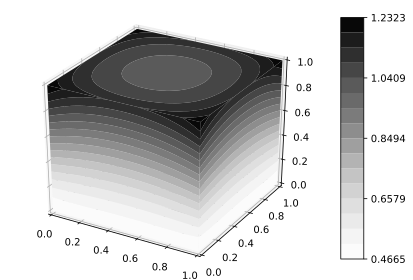
\includegraphics[width=.51\linewidth]{phi.png}
        }
        \caption{Динамика функции $\hat{J}(u)$ по итерациям.}
        \label{cost}
    \end{figure}


    \bibliography{bibliography}

\end{document}

